\section{CoCon Dataset}
\label{sec:cocon}
In this section, we first present our dataset form. Next, we describe data collection process, including text crawling, phrase pre-selecting, annotation, auto-generation and quality control. To better understand our CoCon dataset, we also conduct an analysis on the characteristics of all samples. The dataset collection process is shown in Figure~\ref{fig:framework}. Although the proposed dataset is in Chinese, the methodology can be easily extended to other languages.

\begin{figure}
	\centering
	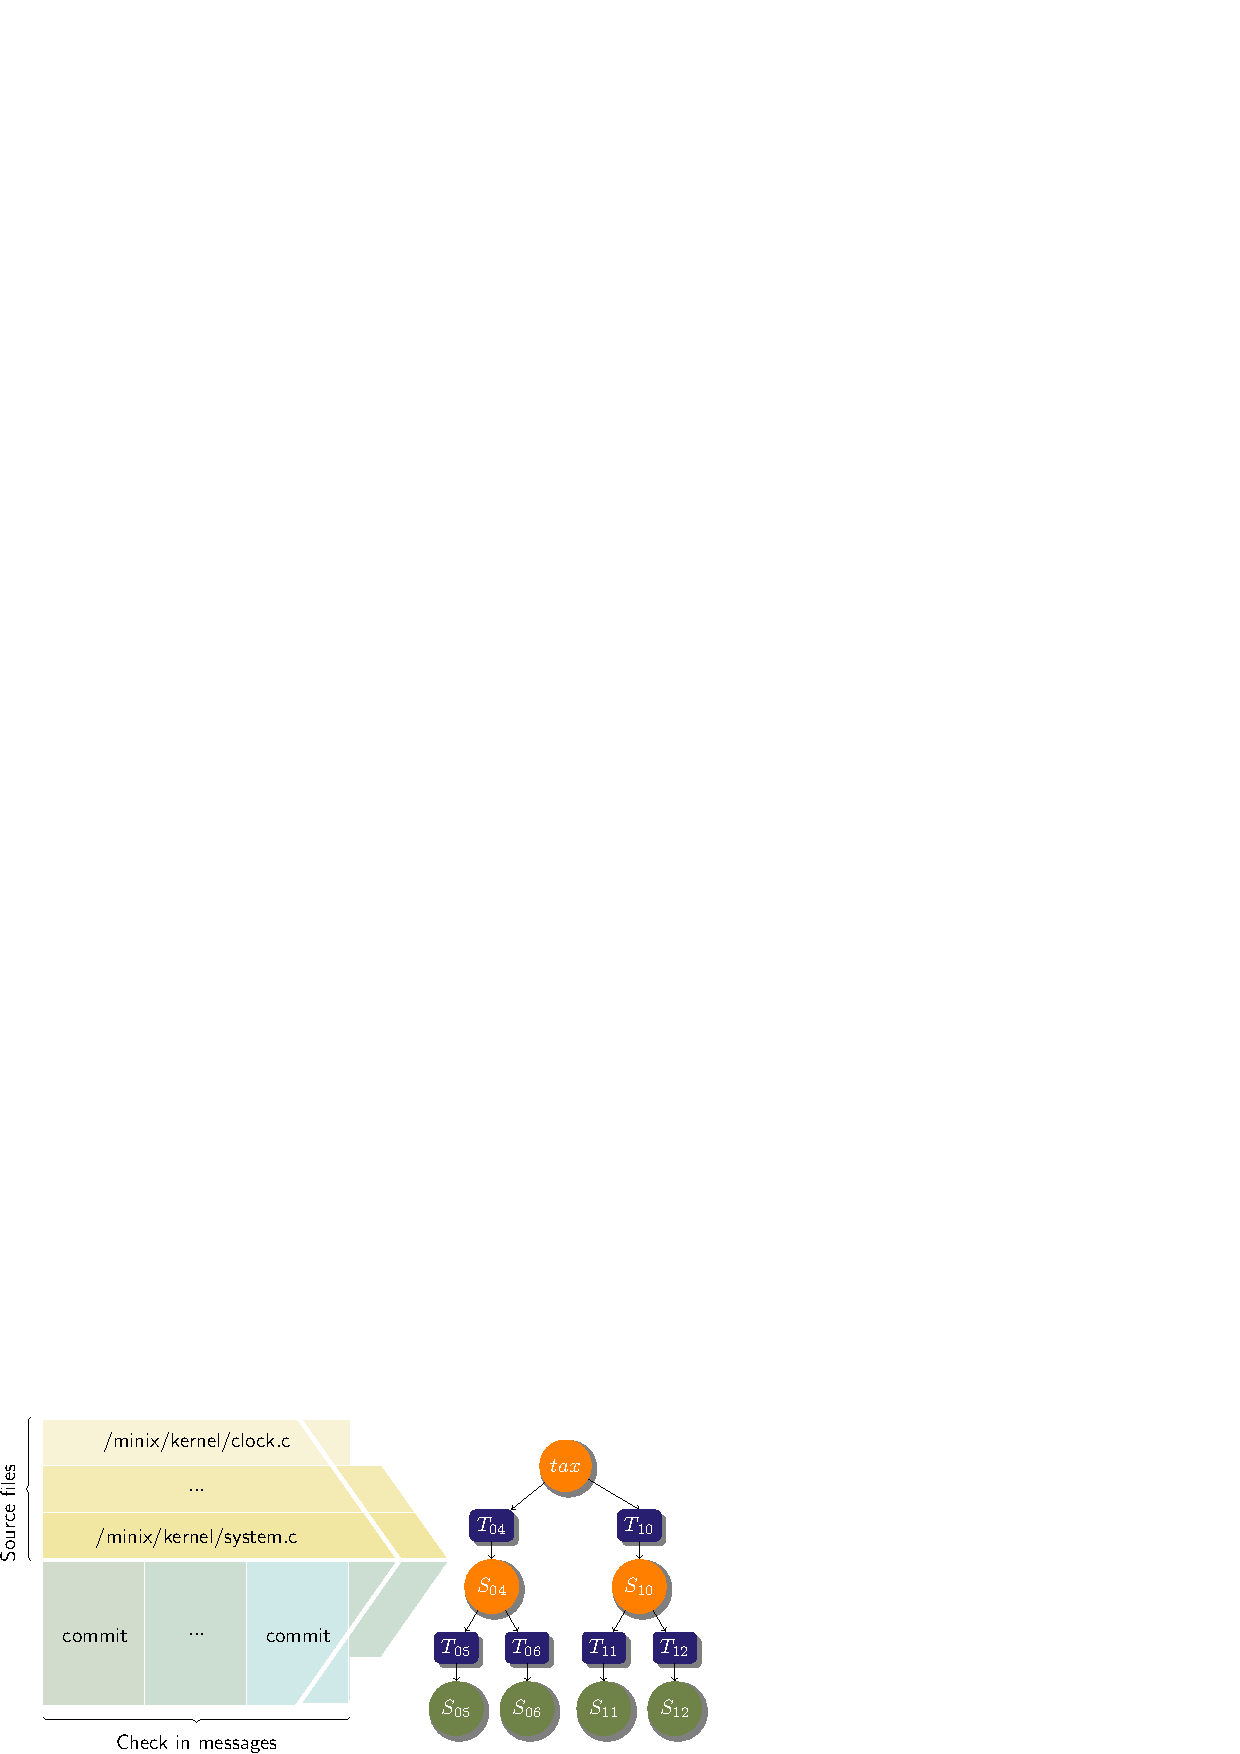
\includegraphics[width=\columnwidth]{images/framework.pdf}
	\caption{CoCon dataset collection process}
	\label{fig:framework}
\end{figure}

\subsection{Dataset Introduction}
Each instance in our CoCon dataset is a triple: $\{p_1, p_2, l\}$, where $p_1$ and $p_2$ are two similar phrases sharing most words, focusing on the same subject
but with different modifiers.
%However, only one of them is plausible by common sense. 
$l$ is the label which indicates the index of the more plausible phrase. 
Therefore, the whole task can be seen as a binary classification problem 
and we use accuracy as evaluation metric. 

In our problem, instead of judging if one phrase is plausible, a pair of phrases are offered to be compared. This is based on that common sense has no absolute criteria. 
Neither can we simply select a threshold for a model to give answer. Hence, we design the task as comparison problem.
%the task as a question of comparison.

\subsection{Raw Data Preprocessing}
%We crawl search queries from a popular e-commerce platform 
%where some noisy and meaningless queries are filtered
%through query normalization including lexical error corrections and query rewriting.

We crawl search queries from a popular Chinese E-commerce platform\footnote{https://www.taobao.com/} and compute lexical and grammatical error corrections using pre-trained neural network. 
We further filter out queries including numbers and English chararacters keeping
those queries composed of only Chinese characters. 
At this point, 4,081,254 common queries remain. 
The length of these queries ranges from 2 to 15, and is 4.73 on average. 
The number of words\footnote{Word segmentations are done by using tools trained 
on E-commerce data in advance.} in queries is distributed between 2 to 8 and 2.07 
on average. 
%The details of character and word number distribution is shown in Figure \ref{fig:wordDist}. 

%\begin{figure}
%	\centering
%	\includegraphics[width=0.95\columnwidth]{images/distributionWords.pdf}
%	\caption{Char and word number distribution of raw data after preprocessing}
%	\label{fig:wordDist}
%\end{figure}


%\subsection{Preprocessed Data Overview}
\subsection{Auto-generation of CoCon pairs}
We define phrases that have commonsense contradiction as \textit{positive samples}, such as ``children's sexy dress" and other phrases as \textit{negative samples} such as ``children's blue dress". 

To have a preliminary and rough understanding over the raw dataset
, we first randomly select 10,000 phrases from preprocessed raw data and do the human annotation. 
Among all selected samples, we find 292 positive samples and 9708 negative samples. It should be noticed that positive samples are much rarer than negative ones, only account for 2.92\%. Obviously, directly annotating the original collection of queries to get more positive samples is not efficient.
%Therefore, we come up with two methods to get expected phrase pairs in CoCon dataset more efficiently: \textbf{Random Replacement} and \textbf{Filter using graph}.
%Therefore, we come up with a method called \textbf{filter using graph} to get expected phrase pairs more efficiently. 


The main idea is that a popular query is more likely to be plausible. 
We propose to construct \textit{Concept Association Graph}, weighted with co-occurrences in the same query between terms by using a large user queries corpus.

%\textit{Step 1: Positive samples preselecting}
\subsubsection{Positive samples preselecting}
%We first crawled user queries on e-commerce platform with data masking among 7 days (2019.07.15-2019.07.21).
We first crawled user queries during 7 days (2019.07.15-2019.07.21) on E-commerce platform after data masking. 
There are 303,285,752 legitimate queries (all Chinese characters with at least
one word) in all. Then we analyze each query to get co-occurrence of each word pair, 
and gradually enrich the graph.
For example, from the query ``sexy blue dress'', we will get three word pairs 
(sexy, dress), (blue, dress) and (sexy, blue). Notice that the edge in our net does not have directions and the word order is neglected.
% in word pairs is of no importance.
Besides, word synonyms are combined together using a Chinese synonym dictionary provided by HIT-SCIR\footnote{https://ltp-cloud.com/download/}.
After construction, the weight of each edge in the graph represents the frequency 
that this word pair was observed in the whole user query corpus. 
A fragment of our constructed \textit{Concept Association Graph} is shown in Figure \ref{fig:net}.

\begin{figure}
	\centering
	\includegraphics[width=0.8\columnwidth]{images/associationNetColor.pdf}
	\caption{A fragment of \textit{Concept Association Graph}}
	\label{fig:net}
\end{figure}

However, the non-uniform user distribution can lead to bias. For example, there may
be more female users than male users. As a result, the frequency of word pair 
(electric, dress) may larger than that of (electric, torch) even though the former
is less plausible.

Mutual information is a suitable criterion to measure the dependency of two words. 
If word A appears $x$ times in the query corpus, word B appears $y$ times, 
the word pair (A,B) appears $z$ times, and the total number of words is $N$, then the mutual information between word A and B is defined as:
\begin{equation}
I(A,B) = log\frac{P_r(A\wedge B)}{P_r(A)\times P_r(B)}
\end{equation}
and can be estimated as:%using:
\begin{equation}
I(A,B) \approx log\frac{z\times N}{(x+z)\times (y+z)}
\end{equation}

We use mutual information to calculate the strength of word associations in 
our constructed graph, which is noted as ``plausibility.''
For a phrase $T=(w_1, ..., w_m)$, %there may be not only two words, 
where there is more than two words, 
we calculate the overall plausibility $P$ as:
\begin{equation}
P(T) = \frac{2}{m*(m-1)}\sum_{i=1}^{m-1}\sum_{j=i+1}^{m}I(w_i, w_j)
\end{equation}

Besides, based on the idea that phrases should be common enough,
we remove the phrase which contains any rare word that appears less than a threshold in our graph.
1 million is set as threshold in our problem as total number of queries are more than 300 millions.   %\KZ{100,000 seems like a very large number!}
%If all word pairs in a phrase doesn't exist in our graph, this phrase will also be filtered. Then, 
The remained phrases are ranked according to their overall plausibility score from small to large to get the most implausible phrase list.

To evaluate the effectiveness of the above method, we test on our 10,000 preliminary annotated phrases. %as example.
After removing rare words, 6,381 phrases (include 94 positive ones) are removed where the rate of positive phrase is 1.47\%. After removing non-exist word pair, another 107 phrases (include 9 positive ones) are removed. Finally, 3,512 phrases (include 167 positive ones) remain. Among top 526 phrases (15\%), 77 positive ones are found, where the rate of positive phrases achieves 15.4\%, %remarkably increases compared to 2.92\% on randomly selected raw data.
achieves a remarkable increase from 2.92\% on randomly selected raw data.
%on the 10,000 randomly selected on preprocessed raw data.
%showing the validity of the constructed graph.

%Therefore, we apply 
Verifying the validity of \textit{Concept Association Graph}, the above method is applied on 
our whole unlabeled preprocessed 4,081,254 phrases,
%top 15\% (1,176,922 phrases) of overall plausibility score are kept. 
we fetch the top 18,000 phrases which have low plausibility score for human annotation due to the 
limited resources.

%\textit{Step 2: Phrase Annotation}
\subsubsection{Phrase Annotation}

This part describes the guideline for annotators: when to ignore a phrase and what kind of implausible phrases do we need.
\begin{enumerate}
	\item Phrases that belong to any one of these three cases can be directly ignored: 
	\begin{itemize}
		\item [-] Plausible phrase.
		\item [-] Absence of a clear subject.
		\item [-] Contains rare word~(i.e., unfamiliar to the annotator)
	\end{itemize}
	\item Judge the phrase to be implausible if it belongs to the following four commonsense contradiction category:
	\begin{itemize}
		\item [-] Several modifiers are contradictory between themselves. %Several modifiers for one subject and commonsense contradiction exists between modifiers. 
		For example, in ``Europe Korean curtain''~(欧韩窗帘), two national modifiers are contradictory.
		
		\item [-] The modifier is contradictory with the intrinsic property of subject. For example, ``vitreous porcelain''~(玻璃青花瓷) and ``children's sexy dress''~(儿童性感连衣裙).%, ``boy night skirt''~(男童睡裙).
		
		\item [-] The modifier is strange for describing the subject %'s intrinsic property 
		according to common sense, such as ``Walking alarm clock''~(会走的闹钟) and ``vacuum keyboard''~(真空键盘).
	\end{itemize}
\end{enumerate}

We distribute these 18,000 fetched phrases to 6 person,
and ask them to pick out intuitively the implausible phrase by their common sense. Finally, 15,567 commonsense contradiction samples are returned, hitting the rate of \textbf{86.48\%}, which is much larger than the original rate of \textbf{2.92\%}.

%\textit{Step 3: Negative Samples Generation}
\subsubsection{Negative Samples Generation}
For each positive phrase, we need to find a relative negative one to form a phrase pair. As human rewriting is costly, 
%Because human rewriting is costly, 
we consider a more efficient way to obtain negative samples with the help of our crawled preprocessed query set by using the \textit{concept Association Graph}.
%Because human rewriting is costly, we consider a more efficient way to obtain the associated negative sample given a positive one.
%(plausible one) 
%for each collected commonsense contradiction sample. The plausibility score $P$ is reused in this part: for each positive sample,
%(commonsense contradiction one)
%we pair it with a short phrase in our total preprocessed query data that satisfies the following rules:
For each human-annotated positive sample, we find a query which simultaneously:% satisfies:
\begin{itemize}
	\item Describes the same object.
	\item Possesses the same number of chars.
	\item Only one word in the original positive sample is replaced. %Only one word different from the original positive sample according to the result of segmentation.
	\item Plausibility score is higher than the positive sample.
\end{itemize}

This automatic generation helps us to get 12,416 phrase pairs.% of short phrases.

%\subsection{Additional Verification}
%\subsection{Dataset Validation}
\subsection{Quality Control}
For further improving the quality of dataset, we ask different crowd workers to judge which phrase is more plausible or can not distinguish between two phrases. We also set 300 checking problems. %The annotated pairs 
Answers from annotators who choose correctly on more than 80\% checking problems will be counted into the final collection. Figure \ref{fig:crowd} is the crowd-sourcing web interface of data quality control.%\JQ{right?}

\begin{figure}
	\centering
	\includegraphics[width=0.95\columnwidth]{images/crowdPage.pdf}
	\caption{The crowd-facing web interface used to control quality of dataset}
	\label{fig:crowd}
\end{figure}

During validation, each sample is judged by 5 persons, and those pairs that gain more than 4 same votes are kept. %After this step, 
We finally obtain our \textbf{CoCon} (\textbf{Co}mmonsense \textbf{Con}tradiction) dataset, which contains 9,229 short phrase pairs \footnote{CoCon dataset can be found at \url{http://release_after_acception}}.

